\documentclass[11pt,a4paper]{article}

\usepackage[utf8]{inputenc}
\usepackage[T1]{fontenc}
\usepackage{geometry}
\usepackage{graphicx}
\usepackage{float}
\usepackage{tikz}
\usetikzlibrary{arrows.meta, positioning, shapes.geometric, fit, backgrounds}
\usepackage{hyperref}
\usepackage{array}
\usepackage{booktabs}
\usepackage{longtable}

\geometry{margin=2.5cm}
\setlength{\parindent}{15pt}
\setlength{\parskip}{0pt}
\sloppy

\hypersetup{
  hidelinks,
  pdftitle={Shattered Bytes Final Report},
  pdfauthor={Simone Romano}
}

\newcommand{\projecttitle}{Shattered Bytes}

\begin{document}
\pagenumbering{gobble}
\begin{titlepage}
    \centering
    \vspace*{1.5cm}

    
\includegraphics[width=0.4\textwidth]{img/logo1.jpg}\\[1cm]
    {\LARGE \textsc{Politecnico di Torino}}\\[1.5cm] 

    \vspace{2cm} 
    
    \vspace{0.4cm}
    {\Huge \bfseries Shattered Bytes}\\
    \vspace{0.3cm}
    {\Large \bfseries A Process-Oriented Serious Game for Manual Data Carving}\\
    \vspace{0.2cm}

    \vspace{3cm}


    \vfill
    \large{Simone Romano}\\
    \textit{s344024}\\
    \vspace{1cm}

    

    \begin{flushleft}
    \centering
        \begin{tabular}{cc}
        Prof. Andrea Atzeni
        \end{tabular}
    \end{flushleft}

    \vspace{1cm}

\end{titlepage}

\thispagestyle{empty}
\newpage
\pagenumbering{arabic}
\tableofcontents
\newpage

\begin{abstract}
\projecttitle{} is a browser-based serious game developed for the Computer Forensics and Cyber Crime Analysis course. The project focuses on manual data carving and low-level evidence recovery, but it intentionally avoids presenting the topic as a simple exercise in signature matching. The player acts as a junior forensic analyst involved in a fictional ransomware investigation, Operation Shattered Meridian, and must recover relevant artefacts from raw byte dumps while preserving a defensible investigative process.

The game compresses several forensic concepts into a short interactive campaign: evidence intake, file signature validation, fragmented recovery, relevance triage, MBR offset calculation, weak XOR obfuscation, partial recovery, final reporting, and incident reconstruction. The target duration is approximately 10 to 15 minutes. The main contribution of the project is the integration of byte-level technical tasks with process-oriented assessment. The player is not evaluated only on completion, but also on precision, hint usage, trial-and-error behavior, procedural decisions, reporting discipline, and ability to connect recovered artefacts into a coherent incident chain.
\end{abstract}

\section{Introduction}

This report documents the design, implementation, and educational rationale of \projecttitle{}, a serious game centered on data carving and digital evidence recovery. The project was developed as an individual homework for the Computer Forensics and Cyber Crime Analysis course.

The initial theme of the project was deliberately narrow: manual data carving. This narrowness was also the main design risk. If the game had only asked the player to search for a file header and carve the following bytes, it would have produced a superficial exercise rather than a serious training experience. The project therefore evolved around a stricter requirement: file signatures may appear in the game, but they must never be the whole game.

The final product is a six-act browser game in which the player works through a ransomware investigation. The player receives raw dumps, identifies candidate evidence, selects byte ranges, reconstructs fragments, reasons about partition structures, decodes weakly obfuscated payloads, reports recovery status, and finally arranges recovered artefacts into the incident chain. The game is intentionally compact, but each act introduces one additional complication that forces the player to move from recognition toward reasoning.

\section{Project Goals}

The approved project direction established five main goals. First, the game should avoid a simplistic treatment of signature matching. Second, it should include scenarios with increasing difficulty and realistic forensic complications. Third, it should cover fragmentation, partial recovery, and basic anti-forensics. Fourth, it should discourage blind trial-and-error through a dynamic scoring model. Fifth, it should produce a final result that indicates the level of mastery demonstrated by the player.

These goals shaped both the campaign and the interface. The game is not a collection of unrelated puzzles: every act belongs to the same fictional case, and each recovered artefact gives investigative meaning to the next one. The player is asked to recover files, but also to decide whether a file is relevant, whether a recovery is complete, whether a selected range is defensible, and whether a conclusion is supported by the evidence.

\section{Educational Problem}

Data carving is often introduced through magic numbers: a PNG begins with a recognizable header, a JPEG has a known start and end marker, and so on. This is a useful entry point, but it can create a wrong mental model. A beginner may conclude that forensic recovery is mostly a search operation, while practical analysis requires a much richer workflow.

Several problems are hidden by overly simple exercises. A valid header may be a decoy. A file may be fragmented across non-contiguous regions. Bytes located between two useful fragments may be unrelated residue. A recovered file may be technically valid but irrelevant to the case. A storage structure may need to be interpreted before the evidence becomes visible. An obfuscated artefact may not be searchable in plaintext. A partial recovery may still be valuable, but only if the analyst reports its limits honestly.

\projecttitle{} addresses this educational problem by turning carving into an investigative workflow. The player begins with signatures, but quickly encounters cases where signatures are not enough. The purpose is not to reproduce a full professional forensic suite. The purpose is to make the student practice the small reasoning steps that separate a defensible recovery from a lucky extraction.

\section{Theoretical Background}

The project is based on the idea that a serious game should not merely decorate a traditional exercise with points and graphics. Its educational value depends on whether the game mechanics require the same reasoning processes that the course wants to develop. In this sense, \projecttitle{} treats gameplay as a form of situated practice: the student is placed inside a simplified professional situation and must act through the available tools, constraints, and evidence.

The relevant learning model is closer to apprenticeship than to memorization. A novice forensic analyst does not become competent by only reading the definition of a magic number or the structure of an MBR entry. Those concepts become meaningful when they are used to solve a concrete problem: deciding where evidence starts, where it ends, whether it is complete, and whether it supports a conclusion. The game therefore gives the player partial information, controlled tools, and feedback after action.

\subsection{Situated Learning}

Situated learning assumes that knowledge is strongly connected to the context in which it is applied. A file signature learned in isolation is a static fact. A file signature encountered inside a noisy dump is a forensic clue. The difference is important. The player must decide whether the clue belongs to relevant evidence, whether it is a false positive, and whether the file boundaries are complete.

The game uses a fictional ransomware investigation to create this context. The narrative does not replace the technical task; it gives the technical task an investigative purpose. The player is not asked to recover a PNG because PNGs are convenient. The player recovers a chat screenshot, a forged identity document, an ATM frame, a bank transfer record, a malware payload fragment, and credentials because each artefact answers a question in the case.

\subsection{Experiential Learning}

The game follows an experiential learning cycle. The player performs an action, observes the result, adjusts the hypothesis, and tries again with more precise reasoning. For example, a broad byte selection may still carve something, but it can lower the score or fail validation. A wrong report may be accepted as an action, but it is recorded as weak reporting discipline. A hint can help, but it reduces the final score.

This structure encourages reflection. The player learns not only that a certain command works, but why a forensic action must be exact. The system makes imprecision visible. This is essential for data carving, where a visually plausible recovery can still be methodologically weak if the selected byte range includes unsupported data.

\subsection{Scaffolding and Progressive Difficulty}

Scaffolding is the controlled support given to a learner while they acquire a new skill. In \projecttitle{}, scaffolding appears in three forms. The first is level progression: each act adds one new complication while preserving earlier skills. The second is interface constraint: the player receives only the tools needed for the intended reasoning path. The third is the hint system: hints begin as conceptual orientation and become more operational only if the player asks for additional help.

The progression is deliberate. Act 1 introduces signatures and exact boundaries. Act 2 adds fragmentation. Act 3 adds relevance. Act 4 adds storage-structure reasoning. Act 5 adds obfuscation and partial recovery. Act 6 requires synthesis. This sequence prevents cognitive overload while still moving beyond a single technique.

\subsection{Assessment for Learning}

The assessment is designed as feedback, not only as grading. A simple success/failure result would hide important differences between players. One student may recover the correct artefact after a disciplined search, while another may recover it after many unsupported selections and repeated carving attempts. Both technically finish, but they have not demonstrated the same level of mastery.

The game therefore records process signals: searches, selected ranges, stash operations, carve attempts, reports, hints, and procedure mistakes. These signals become a mastery profile. The profile is useful because it tells the student what kind of forensic behavior they demonstrated: precise selection, weak fragment reconstruction, strong obfuscation handling, poor reporting, or excessive trial-and-error.

\section{Forensic Theory Represented in the Game}

The theoretical core of the game is the distinction between data recovery and defensible evidence recovery. Recovering bytes is not enough. A forensic analyst must explain why those bytes are evidence, why the selected range is justified, and what limitations remain.

\subsection{Data Carving Beyond Signature Matching}

Data carving is the recovery of files from raw data without relying on normal file-system metadata. Signature matching is often the first step because many file formats expose recognizable headers and footers. However, signature matching alone is incomplete. A header may be isolated, corrupted, duplicated, or intentionally planted as a decoy. A file may also be fragmented, so a contiguous selection from header to footer may include unrelated data.

The first acts of the game use this exact distinction. The player can search for recognizable patterns, but must validate the candidate through boundaries, context, and rendered output. This models the idea that signatures generate hypotheses, not conclusions.

\subsection{Fragmentation and Logical Reconstruction}

Fragmentation is one of the main reasons data carving becomes non-trivial. A file may survive deletion in multiple non-contiguous regions. The physical order of bytes on disk is not automatically the logical order of the file. In addition, bytes between fragments may belong to other deleted data or random residue.

The game turns this concept into a workbench mechanic. The player must stash fragments separately and compose them. This is more than an interface convenience: it represents the analytical separation between identifying a fragment and reconstructing the original logical stream.

\subsection{Storage Structures and Offset Reasoning}

Computer forensics often requires reasoning about storage structures before content can be interpreted. An MBR partition table is not evidence in the same way an image is evidence, but it can describe where relevant content starts. Understanding endianness, LBA values, and byte offsets is therefore part of the path from low-level data to useful artefact.

Act 4 was designed to make this reasoning unavoidable. The player cannot simply search for the target image inside a locked region. They must interpret the storage clue, calculate the correct offset, and only then return to carving. This forces the conceptual order used in real analysis: understand the layout before interpreting the content.

\subsection{Anti-Forensics and Uncertainty}

Anti-forensics is represented in simplified form through decoys, locked regions, XOR obfuscation, and missing tails. The goal is not to teach advanced malware analysis, but to introduce the idea that evidence can be hidden, misleading, or incomplete.

The key theoretical lesson is uncertainty management. A partial recovery may still support an investigation, but it must be reported as partial. This distinction is central to forensic defensibility. The game penalizes overclaiming because an analyst who reports an incomplete artefact as fully recovered is producing a stronger conclusion than the evidence supports.

\subsection{Reporting as an Analytical Step}

Reporting is not treated as a final decoration. The terminal report command requires the player to classify the recovery status. The final incident board requires the player to place artefacts into a coherent chain. These mechanics represent the final transformation from recovered data to forensic finding.

The player therefore practices two levels of reasoning: technical reasoning about bytes and interpretive reasoning about evidence. Both are necessary. A technically correct carve is weak if reported incorrectly; a plausible story is weak if not supported by precise recovery.

\section{Narrative Framework}

The game is framed as Operation Shattered Meridian. A regional hospital network has been attacked by the Night Meridian ransomware cell. The live breach is contained, but the payment channel, mule identities, cash-out trail, malware payload, and exfiltrated credentials remain hidden inside seized devices.

The player takes the role of a junior forensic analyst assigned to Agent Root. This narrative role is intentionally modest. The player is not a cinematic hero, but a trainee analyst working through evidence under supervision. The story provides motivation for the technical tasks: the player is not asked to carve arbitrary files, but to recover artefacts that answer specific investigative questions.

The campaign progresses as follows.

\begin{longtable}{p{0.13\textwidth}p{0.25\textwidth}p{0.50\textwidth}}
\toprule
\textbf{Act} & \textbf{Title} & \textbf{Narrative role} \\
\midrule
1 & Intake and False Lead & Recover a deleted ransom-chat screenshot from a seized laptop. \\
2 & The Fracture & Reconstruct a forged identity scan used by a money mule. \\
3 & Signal and Noise & Identify an ATM surveillance artefact among recoverable but irrelevant files. \\
4 & Partition Archaeology & Recover a fraudulent transfer screenshot hidden behind an MBR-derived offset. \\
5 & The Obscured Tail & Decode a partial ransomware payload fragment and report it carefully. \\
6 & Ransomware Aftermath & Reconstruct exfiltrated credentials from XOR-protected fragments. \\
\bottomrule
\end{longtable}

The narrative is functional rather than decorative. It gives the player a reason to care about relevance, order, and reporting discipline. It also supports the final reconstruction board, where recovered artefacts are no longer isolated files but pieces of one incident.

\begin{figure}[H]
\centering
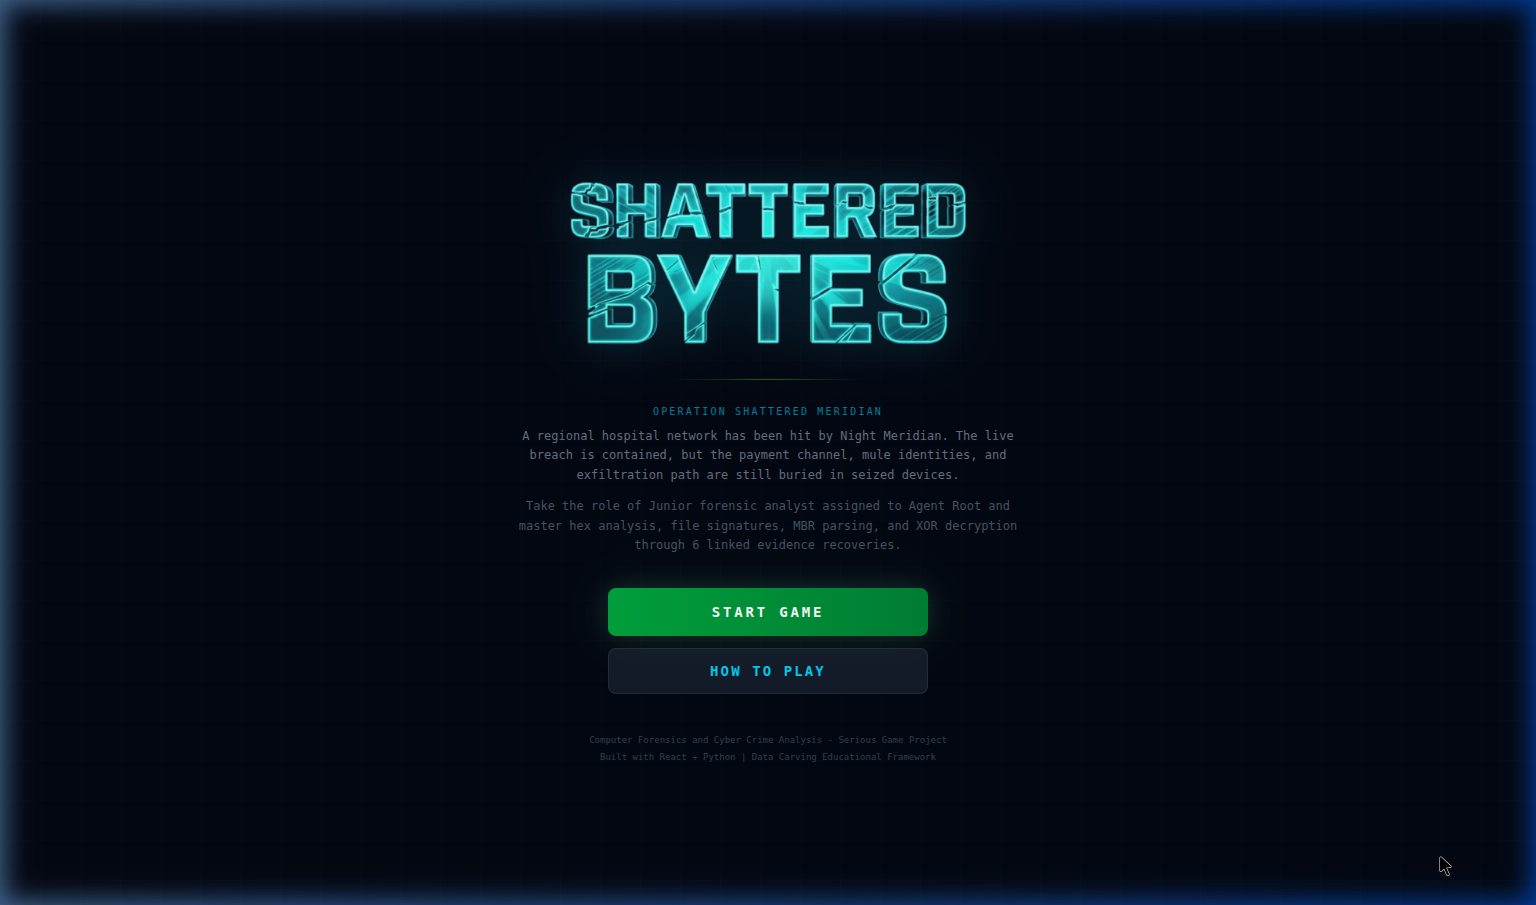
\includegraphics[width=0.85\textwidth]{img/main_menu.png}
\caption{Main menu screen. The player is introduced to Operation Shattered Meridian and can start the campaign or read the tutorial.}
\label{fig:main_menu}
\end{figure}

\section{Gameplay Structure}

The game begins before the hex editor. The first interaction is an evidence intake sequence in which the player places a sealed drive, write blocker, forensic workstation, and hash verification step in the correct order. This establishes the idea that evidence recovery must begin with preservation of integrity. The player then enters the main investigation interface.

Each act uses a common workspace. The hex editor exposes the raw dump and supports byte selection. The terminal provides controlled commands for search, navigation, selection, XOR utilities, hints, and reporting. The workbench stores selected fragments and allows the player to assemble them before carving. The asset viewer renders recovered images or text artefacts, making validation visible. The objectives panel tracks task progress, while the final score system records the player's method.

The interface is designed around constraints. It does not give the player a complete forensic tool. It gives only enough functionality to practice the concepts selected for the course topic. This keeps the game short enough for classroom use and makes the player's reasoning observable.

\begin{figure}[H]
\centering
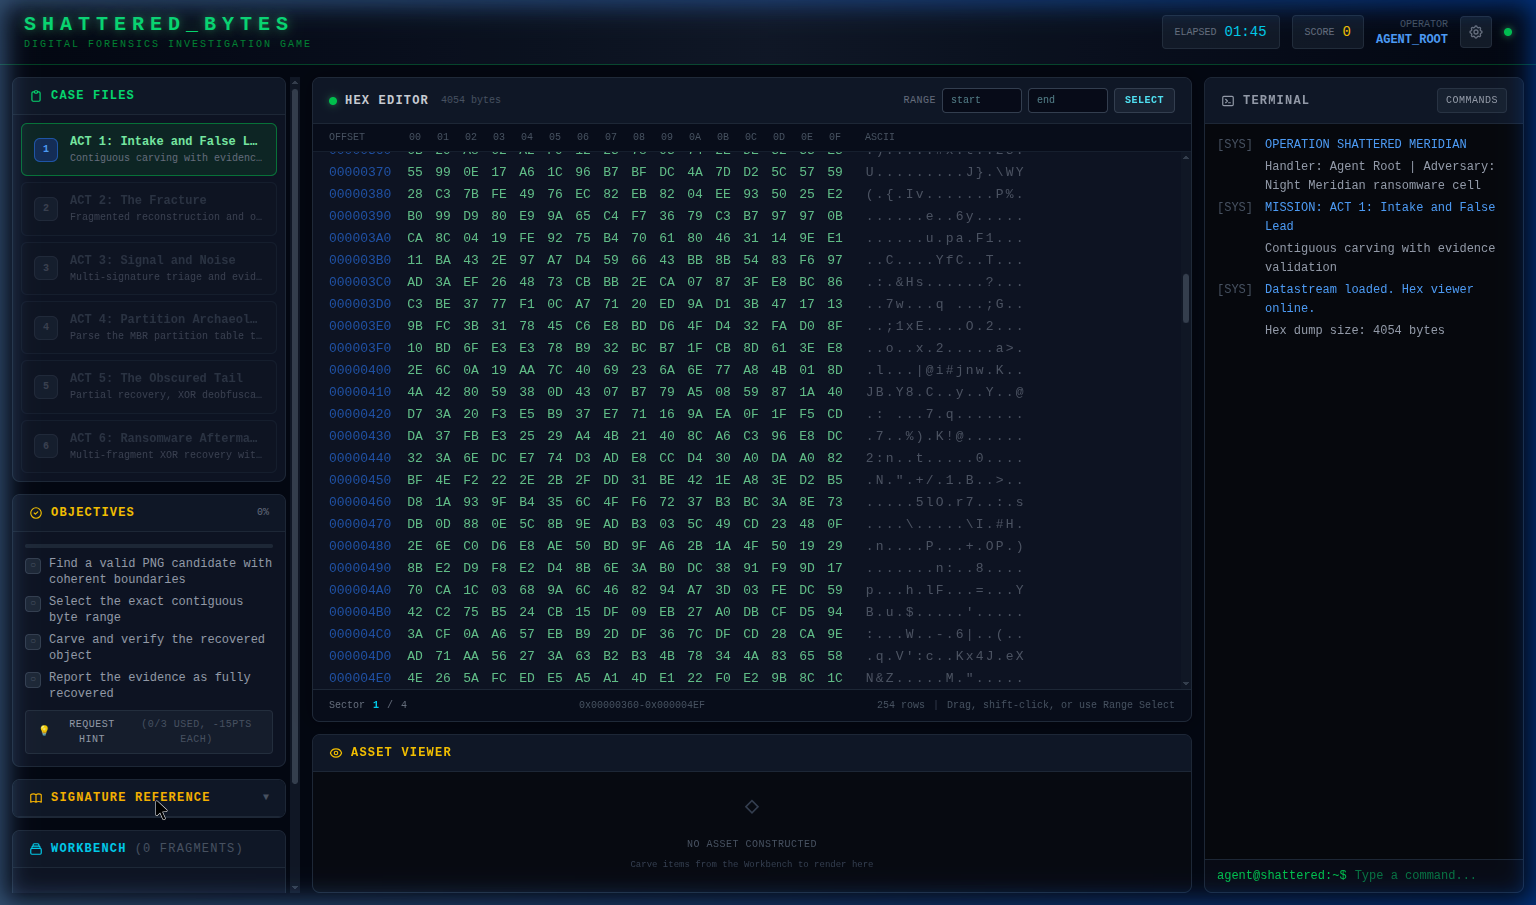
\includegraphics[width=\textwidth]{img/gameplay_interface.png}
\caption{Main investigation interface during Act 1. Left panel: case files and objectives. Centre: hex editor with offset, hex, and ASCII columns. Bottom centre: asset viewer for rendering carved evidence. Right panel: forensic terminal with system messages. The signature reference and workbench panels are collapsed at the bottom left.}
\label{fig:gameplay_interface}
\end{figure}

\subsection{Evidence Intake}

The evidence intake sequence is a drag-and-drop procedure check. The correct chain is:

\begin{center}
\begin{tabular}{cl}
\toprule
Step & Item \\
\midrule
1 & Sealed evidence drive \\
2 & Write blocker \\
3 & Forensic workstation \\
4 & Hash verification \\
\bottomrule
\end{tabular}
\end{center}

This stage is not a quiz in the abstract. It is an interaction that models a simplified acquisition workflow. The player can make mistakes, and those mistakes contribute to procedure risk. The game therefore connects technical recovery with chain-of-custody discipline.

\begin{figure}[H]
\centering
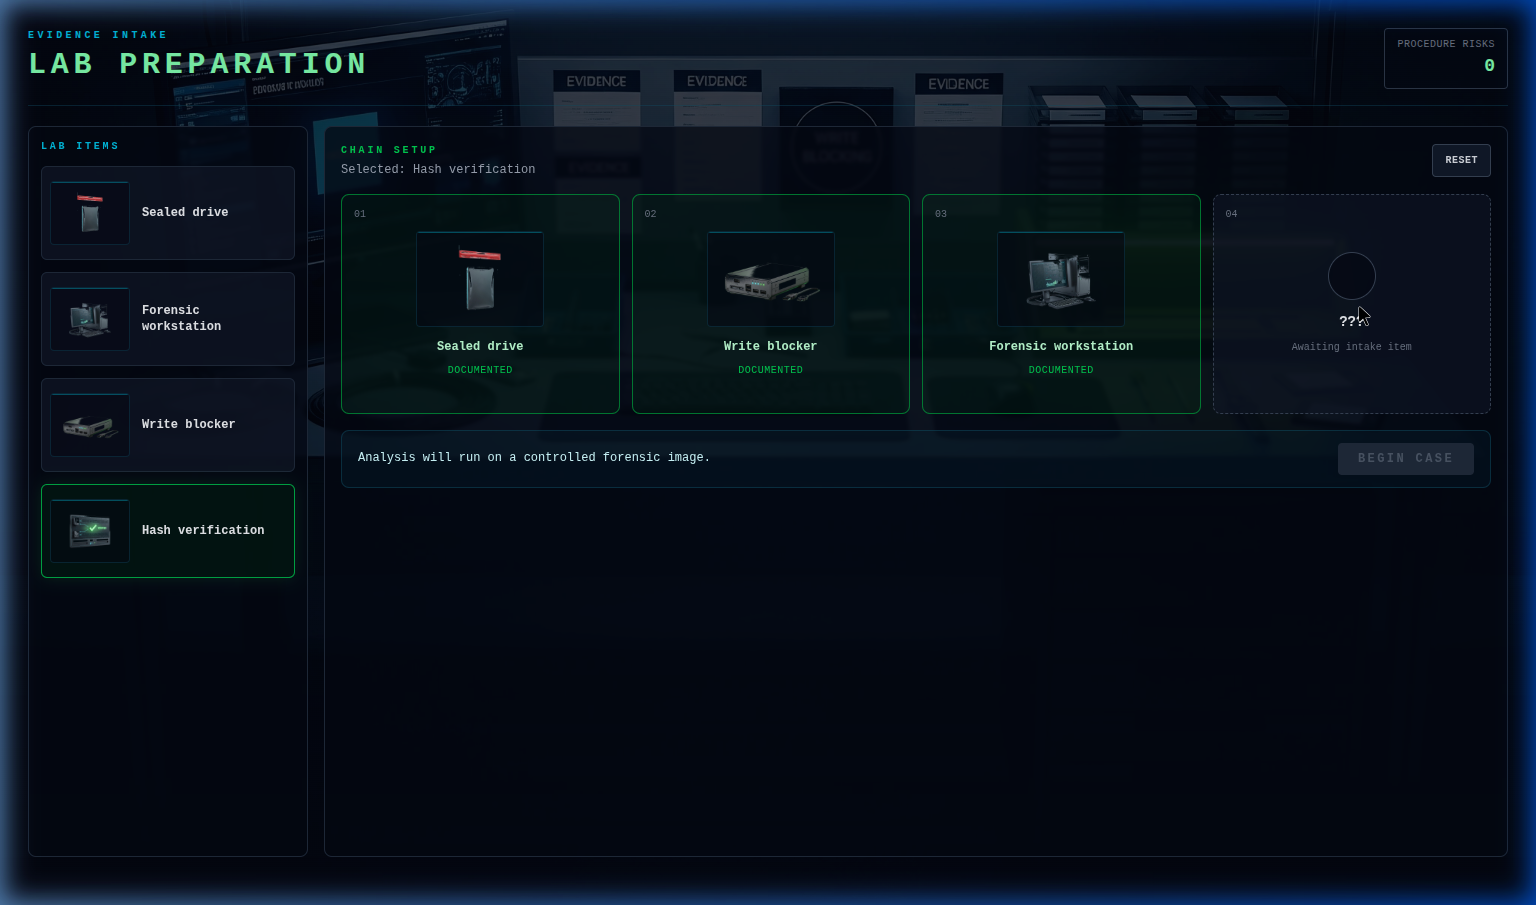
\includegraphics[width=0.85\textwidth]{img/evidence_intake.png}
\caption{Evidence intake screen. The player must place the sealed drive, write blocker, forensic workstation, and hash verification in the correct order. Incorrect ordering increases procedure risk.}
\label{fig:evidence_intake}
\end{figure}

\subsection{Investigation Acts}

The six acts share a common loop: inspect the dump, identify candidates, select a precise range, stash or compose evidence when needed, carve, validate, and report. The loop is repeated with increasing complications. This repetition helps the player internalize the workflow, while the complications prevent the game from becoming mechanical.

\begin{figure}[H]
\centering
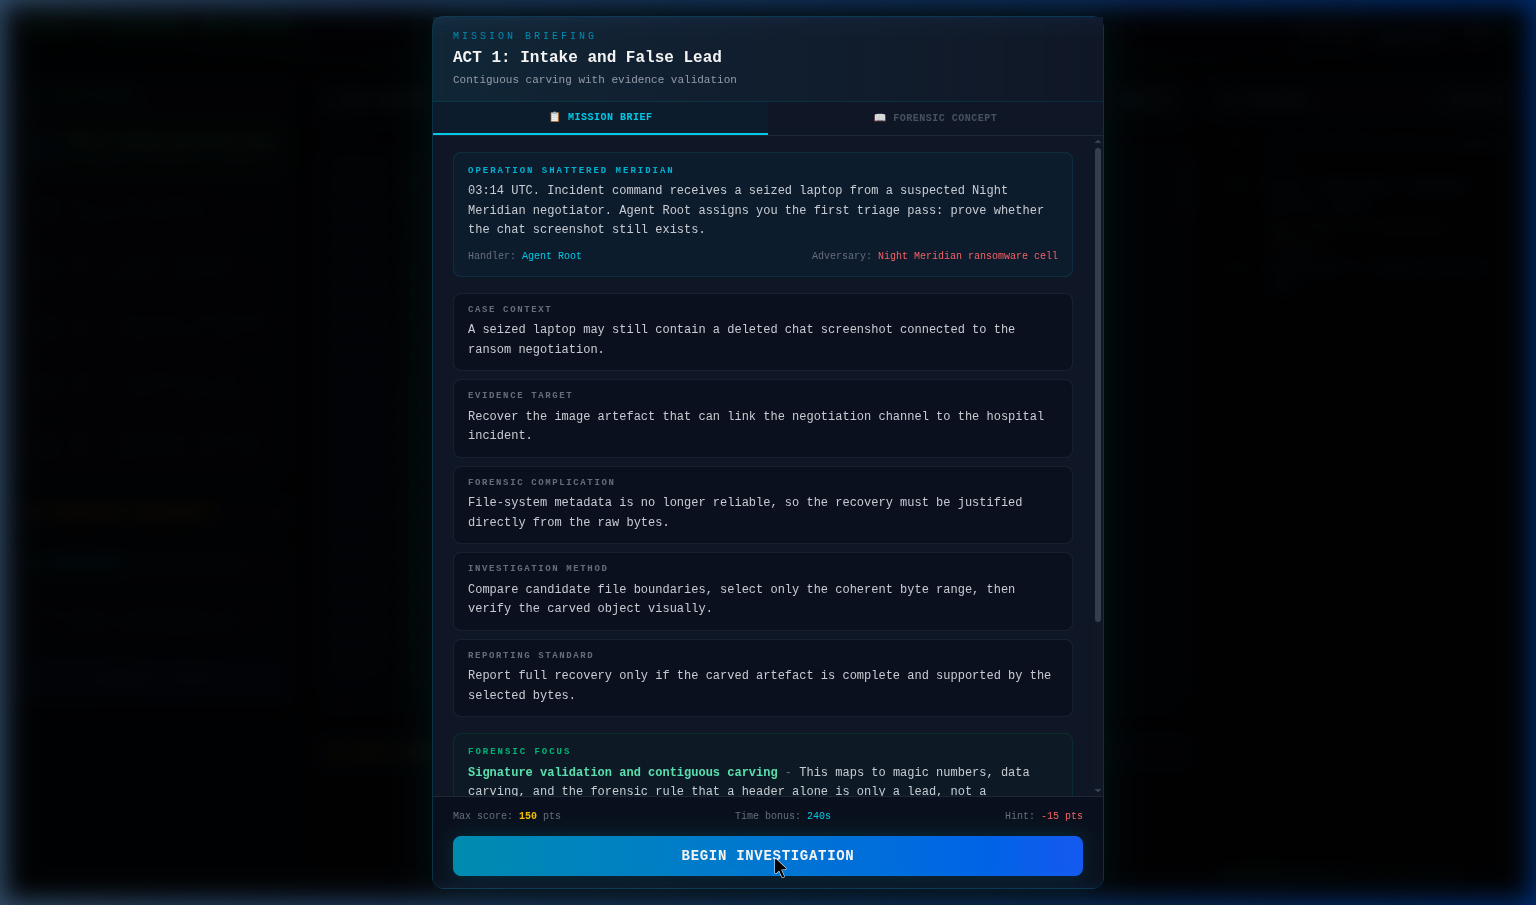
\includegraphics[width=0.85\textwidth]{img/mission_briefing.png}
\caption{Mission briefing for Act 1. Each briefing is structured into case context, evidence target, forensic complication, investigation method, and reporting standard. The forensic focus section maps the act to course concepts.}
\label{fig:mission_briefing}
\end{figure}

\subsection{Final Incident Reconstruction}

After completing the technical acts, the player arranges the recovered artefacts into the incident chain. This final board links the ransom chat, forged identity, ATM frame, bank transfer, malware payload, and credential dump. The goal is to reinforce that recovery is not the end of an investigation. Evidence becomes useful when it supports a coherent and defensible reconstruction.

\section{Level Design}

Each act was designed around one new competency. Earlier competencies remain relevant in later acts, so the final level becomes a synthesis rather than a separate puzzle.

\subsection{Act 1: Intake and False Lead}

The first act introduces contiguous carving. The player must locate a valid PNG candidate, reject a false lead, select the exact range, carve the image, and report full recovery. The act teaches that a file signature is only a lead. A defensible recovery requires coherent boundaries and validation of the carved object.

The design intentionally includes a false candidate. Without it, the level would only test whether the player can search for a magic number. With it, the player must compare candidates and ask whether the byte range behaves like a complete file.

\subsection{Act 2: The Fracture}

The second act introduces fragmented recovery. The target image is split into two surviving byte runs. The player must interpret fragment descriptors and adjacent length information to select only the bytes that belong to each fragment. Bytes between the fragments are unrelated residue and must be excluded.

This act targets a common beginner mistake: assuming that physical proximity implies logical membership. The workbench makes reconstruction explicit by forcing the player to stash fragment payloads and compose them in logical order.

\subsection{Act 3: Signal and Noise}

The third act introduces relevance triage. The dump contains multiple recoverable artefacts, but the case question asks for evidence that can visually support an ATM cash-out hypothesis. The player must recover the artefact that answers the investigative question, not simply the first valid file found.

The act therefore separates technical recoverability from evidentiary relevance. This is important because forensic work is not only extraction; it is extraction in response to a question.

\subsection{Act 4: Partition Archaeology}

The fourth act introduces storage-structure reasoning. The target evidence is hidden behind a locked region. The player must use MBR information, interpret a little-endian LBA value, convert it into a byte offset, and unlock the correct sector before carving.

The design prevents the player from bypassing the reasoning step by searching inside encrypted or locked memory. This forces the intended path: first understand the storage structure, then access the evidence. The act connects byte-level carving with partition-table interpretation.

\subsection{Act 5: The Obscured Tail}

The fifth act introduces weak obfuscation and partial recovery. The payload is XOR-obfuscated and incomplete. The player must use nearby markers to locate candidates, derive a key using known-plaintext reasoning, test coherence, reject a decoy, and report the surviving data as partial.

This act is deliberately not a cryptography exercise. Single-byte XOR is used because it is simple enough to reason about in a short game. The learning objective is to show that evidence may be present but not directly readable, and that incomplete evidence must not be overclaimed.

\subsection{Act 6: Ransomware Aftermath}

The final act combines fragmentation, record structure, decoy rejection, XOR deobfuscation, and incident-response relevance. The player must identify genuine staging records, use length information to determine fragment boundaries, derive the XOR key, decrypt the assembled payload, and recover credentials.

The act is designed as a synthesis. It requires the player to reuse lessons from Act 2, Act 3, and Act 5 in a single workflow. It also closes the narrative by linking the technical recovery to the exfiltration path.

\section{Hint Design}

The hint system was redesigned several times. Early versions either gave too much away or interrupted the player with pop-up guidance. The final version uses on-demand terminal hints and score penalties.

Hints follow a gradual model inspired by puzzle games. The first hint usually changes the player's perspective without naming the solution. The middle hints narrow the reasoning space. The last hint provides a concrete operational direction, but it still expects the player to execute the forensic step correctly.

For example, Act 4 does not immediately tell the player the exact offset. It first suggests that the storage layout is the clue, then points toward the partition table, then reminds the player about LBA and little-endian interpretation, and only later explains that the terminal expects a byte offset. This progression is meant to preserve agency while preventing frustration.

Hints carry a score penalty. This makes assistance available without making it free. A player who solves independently obtains a stronger mastery profile than a player who relies heavily on guidance.

\section{Assessment Model}

The assessment model is process-oriented. The game evaluates not only whether the player finishes a level, but how the player reaches the conclusion. This was a core requirement of the project because a serious game should indicate the player's level of mastery rather than only produce a pass or fail result.

Each act has a maximum score based on difficulty. The level score is affected by correct recovery, selected byte precision, elapsed time, hint usage, bad selections, extra carve attempts, incorrect report attempts, and procedure mistakes. The simplified scoring model is:

\begin{verbatim}
levelScore =
  maxScore
  - 15 * hintsUsed
  - 25 * badSelections
  - 30 * extraCarveAttempts
  - 40 * wrongReportAttempts
  - 15 * procedureMistakes
  + timeBonus
\end{verbatim}

The penalties are not arbitrary decorations. Each one corresponds to a forensic behavior. Bad selections indicate imprecise byte boundaries or unsupported evidence. Extra carve attempts indicate premature extraction before validation. Wrong reports indicate overclaiming or misclassification. Hint usage indicates reliance on external support. Procedure mistakes indicate weak process discipline.

At the end of the campaign, the final mastery report summarizes performance across eight dimensions.

\begin{longtable}{p{0.30\textwidth}p{0.57\textwidth}}
\toprule
\textbf{Dimension} & \textbf{Meaning} \\
\midrule
Signature recognition & Ability to use magic numbers and file boundaries as leads. \\
Offset precision & Ability to select exact ranges and compute byte positions. \\
Fragment reconstruction & Ability to separate logical file content from physical residue. \\
Trial-and-error discipline & Ability to avoid blind carving and unsupported attempts. \\
Obfuscation handling & Ability to reason about XOR and validate decoded output. \\
Procedure discipline & Ability to respect evidence handling and critical process checks. \\
Forensic reasoning & Ability to connect technical findings to case questions. \\
Reporting quality & Ability to distinguish full recovery, partial recovery, and unsupported conclusions. \\
\bottomrule
\end{longtable}

The final mastery label can classify the player as Forensic-ready, Competent examiner, Developing analyst, or Needs remediation. These labels are not professional certifications. They are compact feedback categories that help a student understand where their gameplay showed strength or weakness.

\subsection{Assessment Signals}

The assessment model uses signals that are generated naturally by gameplay. The player does not fill in a separate questionnaire while playing; the game observes the actions required to solve the case. This is important because the objective is not to test vocabulary, but to evaluate whether the player can apply forensic reasoning under constraints.

\begin{longtable}{p{0.23\textwidth}p{0.64\textwidth}}
\toprule
\textbf{Signal} & \textbf{Assessment meaning} \\
\midrule
Search commands & The byte patterns searched by the player reveal whether signatures, markers, and descriptors are being used as reasoned leads or as blind guesses. \\
Navigation commands & Direct jumps and MBR-derived offsets show whether the player can move from logical storage information to physical byte positions. \\
Selections & The start and end offsets of selected ranges show whether recovery boundaries are exact or include unsupported bytes. \\
Stash operations & Saved workbench fragments show whether the player separates relevant payload from descriptors, markers, and residue. \\
Compose attempts & Repeated carving attempts show whether the player validates structure before extraction or tests blindly. \\
XOR operations & Keys and decoded outputs show whether the player applies known-plaintext reasoning instead of brute force. \\
Reports & Terminal conclusions show whether the player distinguishes complete, partial, and unsupported recovery. \\
Procedure checks & Decisions after critical forensic actions show whether the player understands the process implications of the technical step. \\
\bottomrule
\end{longtable}

These signals allow an instructor to inspect the method, not only the result. Two students may both complete a level, but one may do so by selecting exact ranges after a coherent search path, while another may rely on repeated carving, broad selections, and multiple wrong reports. The final score separates these behaviors.

\subsection{Mastery Profile}

The final report shown by the game is intentionally qualitative as well as numerical. A score alone is easy to compare, but it does not tell the student what to improve. The mastery profile therefore groups player behavior into dimensions that correspond to forensic skills.

For example, a player who completes Act 1 and Act 3 quickly may show good signature recognition, but if the same player fails Act 2 and Act 6, the profile will expose weakness in fragment reconstruction. A player who recovers Act 5 but reports it as fully recovered will lose reporting quality even if the byte manipulation was correct. This distinction is central to the project: technical extraction and forensic conclusion are related, but not identical.

\subsection{Anti-Trial-and-Error Design}

The game does not prevent all wrong actions. It allows mistakes because mistakes are useful for learning, but it makes them visible and costly. Broad byte selections, repeated carving, and unsupported reports are accepted as player actions, then reflected in the score and timeline.

This approach is preferable to hard-blocking every wrong action. If the interface simply refused a bad range, the player might learn by constraint rather than by reasoning. Instead, \projecttitle{} lets the player act, records the action, and uses the final feedback to show the cost of imprecision.

\section{Procedure Checks}

Knowledge-check quizzes were initially considered, but they were removed because they duplicated the assessment already present in the gameplay. Instead, the game uses procedure checks at moments where the player has just performed a meaningful forensic action.

The difference is important. A generic quiz asks whether the player remembers a concept. A procedure check asks whether the player understands the action they just performed. For example, after reconstructing fragments, the player may be asked why excluding gap bytes matters. After unlocking an MBR-derived region, the player may be asked why LBA conversion was necessary. After a partial XOR recovery, the player may be asked why the final report cannot claim full recovery.

This approach keeps assessment inside the investigation. It also makes the correlation with course topics stronger without adding detached textual interruptions.

\section{Design Decisions}

Several design decisions were made to keep the game aligned with forensic learning rather than general puzzle solving.

First, the briefing text was standardized across acts. Earlier versions sometimes gave too much information, effectively telling the player what to search. The final briefings separate case context, evidence target, forensic complication, investigation method, and reporting standard. This gives the player a stable reading structure while preserving the need for deduction.

Second, direct shortcuts were removed when they undermined the intended reasoning. In Act 4, direct signature search inside a locked region would allow the player to bypass the MBR calculation. The final design blocks that shortcut so that the storage-structure lesson remains meaningful.

Third, hints were rewritten to be gradual. The first hint should rarely contain a command. It should reframe the problem. Later hints may become operational, but only after the player has had time to reason. This preserves the game feel while preventing dead ends.

Fourth, gameplay mechanics were preferred over textual quizzes when possible. Evidence intake and the final timeline board are examples. They are not merely decorative scenes: they require the player to perform a forensic ordering task, and mistakes are recorded as procedure risk.

Fifth, the game remains deterministic. Randomness would make classroom comparison harder and would complicate debugging. Deterministic levels allow the instructor to know exactly what each student faced, while still leaving room for different solution paths.

\section{Technical Implementation}

\projecttitle{} is implemented as a React and Vite browser application. It does not require a backend service and can be deployed as a static site. This was an intentional choice: the game should be easy to run during laboratory testing and easy to host as a public demo.

\begin{longtable}{p{0.28\textwidth}p{0.60\textwidth}}
\toprule
\textbf{Area} & \textbf{Implementation} \\
\midrule
Frontend framework & React with Vite. \\
Styling & Tailwind CSS and custom interface components. \\
Level data & Deterministic JSON files served from \texttt{public/levels/}. \\
Source assets & Images and videos stored in \texttt{assets/} and \texttt{public/}. \\
Game state & React hooks, mainly the game orchestration logic in \texttt{src/hooks/}. \\
Deployment & Static GitHub Pages build through GitHub Actions. \\
\bottomrule
\end{longtable}

The main source folders are:

\begin{verbatim}
src/components/             UI and gameplay components
src/data/                   campaign, story, signatures, procedures
src/hooks/                  game state and orchestration logic
src/utils/                  byte, buffer, and crypto helpers
public/levels/              generated JSON level files
assets/                     source visuals and media
scripts/level_generation/   deterministic level generation scripts
\end{verbatim}

The level dumps are deterministic. This makes the game repeatable, inspectable, and suitable for classroom use. It also allows the validation logic to compare player selections against known evidence ranges without relying on hidden server-side state.

\subsection{Validation Logic}

Validation is based on explicit level metadata. Each generated level contains the raw dump and the expected evidence regions. When the player selects bytes, stashes fragments, composes a stream, or submits a report, the game compares the action against the expected forensic answer.

This metadata is not exposed to the player during normal gameplay. It exists to make assessment reliable. For example, the game can distinguish between a selection that exactly matches a fragment, a selection that overlaps the fragment but includes extra residue, and a selection that targets a decoy. These distinctions are necessary for meaningful feedback.

\subsection{Technical Boundaries}

The implementation deliberately avoids features that would make the educational model harder to inspect. There is no hidden backend and no adaptive artificial intelligence deciding whether the player is correct. The relevant answers are encoded in deterministic level metadata, and the interface exposes a controlled subset of forensic actions.

This simplicity is a design choice. The objective is not to simulate a full forensic workstation, but to make a specific reasoning path visible. A more realistic toolset could increase authenticity, but it would also make it harder to understand whether the student solved the intended conceptual problem or simply used a powerful automated feature.

\section{Development Process}

The project changed significantly during development. The first versions leaned too heavily on signature matching. The campaign was then redesigned around escalating complications: fragmentation, multi-signature triage, MBR offsets, XOR obfuscation, partial recovery, and final incident correlation.

Several mechanics were removed or rewritten because they weakened the educational objective. Random pop-up hints were removed because they interrupted agency. Knowledge-check quizzes were removed because they felt detached from the investigation. Overly explicit briefings were rewritten so that the player could deduce the solution from the case context rather than receive it directly. Terminal commands that did not contribute to gameplay were removed.

Usability also required several iterations. Long byte selections initially became difficult when the selected range extended beyond the visible hex window. This was addressed by supporting range-based selection and improving drag behavior. The workbench was adjusted to handle multiple fragments more clearly. The asset viewer was fixed to render carved evidence reliably. The intro video was replaced and made browser-compatible with explicit audio enabling. The final report layout was adapted to default browser zoom. GitHub Pages deployment was prepared with relative asset paths.

The latest gameplay additions include the evidence intake sequence and the final incident reconstruction board. These mechanics were added to strengthen the connection between the game and broader forensic practice, so that the player is not only carving files but also preserving evidence and reconstructing an incident.

\section{Relationship With Course Topics}

\projecttitle{} maps to several topics normally discussed in a computer forensics course.

Evidence handling and integrity appear in the evidence intake phase, where the player reconstructs a simplified chain involving a sealed drive, write blocker, forensic workstation, and hash verification. This introduces acquisition discipline before analysis begins.

File-system forensics and data carving appear throughout the campaign. The player works below the normal file-system abstraction and recovers artefacts directly from raw byte dumps. Signatures are used as leads, but every act adds a condition that prevents signature matching from becoming sufficient.

Fragmentation appears in Act 2 and Act 6. The player must distinguish file content from unrelated gap bytes, reconstruct fragments in logical order, and justify exact boundaries.

MBR and low-level storage reasoning appear in Act 4. The player must interpret partition-table information, handle little-endian representation, convert LBA values, and calculate a byte offset before accessing the target area.

Anti-forensics appears through decoys, false positives, locked regions, XOR obfuscation, and partial recovery. These mechanisms are simplified, but they introduce the idea that evidence may be hidden, misleading, or incomplete.

Reporting appears through terminal conclusions, procedure checks, final mastery reporting, and the final incident board. The player must distinguish fully recovered evidence from partial evidence and connect recovered artefacts into a defensible chain.

\begin{longtable}{p{0.30\textwidth}p{0.52\textwidth}}
\toprule
\textbf{Course-related concept} & \textbf{Gameplay implementation} \\
\midrule
Evidence preservation & Evidence intake sequence with sealed drive, write blocker, workstation, and hash verification. \\
Magic numbers & PNG and JPEG recovery paths, with decoys that prevent blind trust in headers. \\
Data carving & Manual range selection, stashing, composing, and asset validation. \\
Fragmentation & Two-run reconstruction in Act 2 and multi-record reconstruction in Act 6. \\
Unallocated residue & Explicit exclusion of gap bytes between useful fragments. \\
MBR and partition tables & Act 4 requires interpreting a partition entry and deriving a byte offset. \\
Little-endian representation & Act 4 forces byte-order reasoning before navigation. \\
Anti-forensics & False leads, locked areas, XOR-obfuscated payloads, and decoy records. \\
Partial recovery & Act 5 requires reporting a recovered fragment without claiming complete evidence. \\
Forensic reporting & Terminal reports, final mastery profile, and incident reconstruction board. \\
\bottomrule
\end{longtable}

\section{Evaluation of Educational Effectiveness}

The game supports educational evaluation at three levels.

The first level is in-game performance. The score and mastery report provide immediate evidence of how the player behaved: whether they selected precise byte ranges, avoided unnecessary attempts, used hints sparingly, handled obfuscation correctly, and reported honestly.

The second level is process traceability. The investigation timeline records searches, selections, stash operations, carve attempts, XOR steps, hints, reports, and procedure decisions. This allows an instructor to inspect not only whether the player succeeded, but how the player approached the task.

The third level is classroom observation. During laboratory testing, students can play the game while the instructor observes where they hesitate, which hints they request, whether they understand the final report, and whether they can explain why a recovery is defensible. This can be complemented with a short post-game questionnaire on clarity, difficulty, engagement, and perceived learning value.

This structure responds to a central concern in serious game evaluation: engagement alone is not evidence of training value. The game must show that the player practiced the intended reasoning. The combination of scoring, mastery dimensions, traceable actions, and post-game discussion makes that evaluation more concrete.

\subsection{Suggested Laboratory Protocol}

The game can be tested during a laboratory session without requiring installation. A possible protocol is the following. First, students receive the live demo link and a short narrative introduction. Second, they play the game individually for approximately 10 to 15 minutes. Third, the instructor asks students to compare final mastery profiles and discuss where they lost points. Fourth, a short debrief connects each act to the corresponding forensic concept.

This protocol keeps the game from becoming only entertainment. The most valuable learning moment may happen after play, when students compare their methods. A student who reached the same artefact with fewer attempts can explain their reasoning. A student who overclaimed a partial recovery can see why the report matters. The game therefore provides concrete material for discussion.

\subsection{Evidence for Didactic Value}

The didactic value of the game can be evaluated through several observable outcomes. Students should be able to explain why a header is not enough for recovery, why fragmented files require exact boundaries, why irrelevant but valid artefacts should not be reported, why MBR offsets must be calculated before carving hidden regions, and why partial recovery must be reported with uncertainty.

The game also produces measurable traces: score, hint usage, wrong selections, carve attempts, procedure mistakes, and final mastery labels. These traces can be collected during a classroom test and compared with students' qualitative feedback. If students enjoy the game but consistently fail to explain the forensic reasoning, the design would need revision. If students can explain their actions and the trace data shows disciplined behavior, the game supports its training claim.

\section{Limitations}

The game intentionally simplifies several forensic realities. The dumps are synthetic and deterministic rather than acquired from real devices. This is necessary to keep the experience short, repeatable, and suitable for classroom testing. The anti-forensic technique is limited to single-byte XOR. This is not meant to represent modern encryption, but to introduce the idea that evidence may be present without being directly readable. The chain-of-custody model is simplified into a short procedural interaction and does not reproduce the full legal and documentary requirements of a real investigation.

The scoring model is also an approximation. It is useful for feedback and comparison between playthroughs, but it should not be treated as a professional certification. A player's mastery profile is an educational signal, not a formal qualification.

\section{Future Work}

Future development could add optional expert levels with larger dumps and more realistic file-system artefacts. A teacher dashboard could expose player timelines in a more readable format. The final mastery report could be exported as a downloadable PDF. Difficulty profiles could allow the same campaign to be used for beginners and more advanced students. A post-game survey could help collect structured feedback during laboratory testing. The narrative could also be expanded into additional branches, such as network artefacts, timeline correlation, or memory-resident evidence.

\section{Conclusion}

\projecttitle{} is a compact serious game designed to teach forensic reasoning through interaction. It begins with accessible data carving and gradually introduces the complications that make forensic work more than pattern recognition: decoys, fragmentation, relevance, storage structures, obfuscation, partial recovery, and reporting.

The final product is both a playable demo and a small training environment. It asks players to recover evidence, justify technical choices, avoid unsupported conclusions, and connect artefacts into an incident narrative. This directly addresses the original project objective: to create a serious game that explores data carving in a nuanced way and provides meaningful feedback on the player's demonstrated mastery.

\end{document}
